\textbf{Notation:} Right-hand side = RHS, Left-hand side = LHS

\vspace{0.2cm}

\colorbox{yellow!30}{\parbox{\dimexpr\textwidth-2\fboxsep}{\textbf{Visual Guide:} \colorbox{yellow!50}{Rules in yellow} are being modified in this step. \textcolor{orange!80!black}{Rules in dark yellow/orange} were just added. \textcolor{gray}{Rules shown in gray} have just been removed.}}

\vspace{0.5cm}

\section*{Original Grammar}

Let's start with this context-free grammar (CFG):
\begin{align*}
    {% for variable, rules in initial_grammar.items() -%}
    {{variable}} &\to {% for rule in rules -%} {{ "\\varepsilon" if rule == 'e' else rule }} {% if not loop.last %} \mid {% endif %}
    {%- endfor %}\\
    {% endfor -%}
\end{align*}

Our goal is to convert this grammar into \textbf{Chomsky Normal Form (CNF)}, which means every production must look like:
\begin{itemize}
    \item $A \to a$ (one variable produces one terminal), or
    \item $A \to BC$ (one variable produces exactly two variables)
\end{itemize}

\vspace{0.3cm}
\noindent\fbox{\parbox{\dimexpr\textwidth-2\fboxsep}{
\textbf{Why CNF?} CNF is useful because it gives us a standardized form that makes parsing algorithms (like the CYK algorithm) much more efficient. Think of it like converting fractions to a common denominator—it makes everything easier to work with!
}}

\section{Step 1: Create a New Start Variable}

{% set ns = namespace(s_found=false) %}
{% for variable, rules in initial_grammar.items() %}
  {% for rule in rules %}
    {% if "S" in rule %}
      {% set ns.s_found = true %}
    {% endif %}
  {% endfor %}
{% endfor %}

\noindent\textbf{The Problem:} {% if ns.s_found %}In the original grammar, $S$ appears on the right-hand side of some productions. In CNF, the start variable should never appear on the RHS—it should only be used to "kick off" derivations.{% else %}Even though $S$ doesn't appear on any RHS in this grammar, we still follow the standard procedure.{% endif %}

\noindent\textbf{The Solution:} Create a brand new start variable $S_0$ (read as "S sub-zero" or "S naught") that only points to the old start variable:

\begin{align*}
    \mathbf{S_0} &\to \mathbf{S}\\
    {% for variable, rules in initial_grammar.items() -%}
    {{variable}} &\to {% for rule in rules -%} {{ "\\varepsilon" if rule == 'e' else rule }} {% if not loop.last %} \mid {% endif %}
    {%- endfor %}\\
    {% endfor -%}
\end{align*}

\noindent\textbf{Think of it like this:} $S_0$ is a "wrapper" around our original grammar. It keeps $S$ protected and ensures we can safely modify the rest of the grammar.

\section{Step 2: Eliminate $\varepsilon$-Rules (Epsilon Rules)}

\subsection{Step 2a: Find Nullable Variables}

\noindent\textbf{What's a nullable variable?} A variable is \textit{nullable} if it can eventually produce the empty string $\varepsilon$ (epsilon). This can happen directly (like $A \to \varepsilon$) or indirectly (like $A \to B$ and $B \to \varepsilon$).

\noindent\textbf{In our grammar, these variables are nullable:}
\begin{align*}
    V_{\varepsilon}=\{ {%- for variable in nullable %} {{variable}} {%- if not loop.last -%} , {% endif -%} {%- endfor -%}\}
\end{align*}

{% if nullable|length > 0 %}
\noindent\textbf{Why does this matter?} Anywhere these variables appear, they might "disappear" (become $\varepsilon$). We need to account for all possibilities.
{% endif %}

\subsection{Step 2b: Analyze Rules Containing Nullable Variables}

Now we examine \textit{every} rule in the grammar to see which ones contain nullable variables. For each rule that contains nullable variables, we need to generate new rules covering all possible cases where those variables "disappear."

\vspace{0.3cm}

{% if nullable_analysis|length > 0 %}
{% for item in nullable_analysis -%}
\begin{tcolorbox}[colback=yellow!5!white,colframe=orange!75!black,title=Analysis of ${{item.variable}} \to {{item.original_rule}}$]

\textbf{Original Rule:} 
{% set rule_str = item.original_rule %}
${{item.variable}} \to {% for i in range(rule_str|length) -%}
{%- if i in item.positions -%}
\colorbox{yellow!50}{${{- rule_str[i] -}}$}
{%- else -%}
{{- rule_str[i] -}}
{%- endif -%}
{%- endfor %}$

\vspace{0.2cm}
\textbf{Nullable Variables in this rule:} $\{ {%- for nv in item.nullable_vars -%}{{nv}}{%- if not loop.last -%}, {%- endif -%}{%- endfor -%} \}$

\vspace{0.2cm}
\textbf{New Rules Generated:}
\begin{itemize}
{% for new_rule in item.new_rules %}
    \item Remove $\{ {%- for rv in new_rule.removed -%}{{rv}}{%- if not loop.last -%}, {%- endif -%}{%- endfor -%} \}$: \quad ${{item.variable}} \to {{new_rule.rule}}$
{% endfor %}
{% if item.new_rules|length == 0 %}
    \item (no valid new rules - would result in empty string)
{% endif %}
\end{itemize}

\end{tcolorbox}

{% endfor -%}

\vspace{0.3cm}
\noindent\textbf{Understanding the analysis:}
\begin{itemize}
    \item \colorbox{yellow!50}{Variables highlighted in yellow} are nullable
    \item Each box shows an original rule and all the new rules we must add
    \item "Remove $\{A\}$" means create a version where $A$ disappears (becomes $\varepsilon$)
    \item If multiple nullable variables exist, we try all combinations
\end{itemize}
{% else %}
\noindent\textbf{Good news!} No rules in the grammar contain nullable variables, so no new rules need to be generated.
{% endif %}

\subsection{Step 2c: Add New Rules for Each Possibility}

For every production that contains a nullable variable, we create additional versions where that variable is "removed" (replaced with nothing). If multiple nullable variables appear, we consider all combinations.

{% if nullable|length > 0 %}
\noindent\textbf{Example:} If ${{nullable[0]}}$ is nullable and we have $A \to {{nullable[0]}}BC$, we add the production $A \to BC$ (where ${{nullable[0]}}$ vanished).
{% endif %}

\noindent\textbf{After adding all these new possibilities:}
\begin{align*}
    {% for variable, rules in e_removal_1_grammar.items() -%}
    {{variable}} &\to {% for rule in rules -%}
    {% if rule == 'e' -%}
        {{ "\\textcolor{gray}{\\varepsilon}" }}
    {% elif rule in rules_with_nullable.get(variable, []) -%}
        \colorbox{yellow!50}{${{- rule -}}$}
    {% elif rule in initial_grammar.get(variable, []) or (variable == 'S_0' and rule == 'S') -%}
        {{ rule }}
    {% else -%}
        \textcolor{orange!80!black}{ {{- rule -}} }
    {% endif -%}
    {% if not loop.last %} \mid {% endif %}
    {%- endfor %}\\
    {% endfor -%}
\end{align*}

Notice the rules in yellow contain nullable variables, and the rules in dark yellow/orange are the newly added possibilities!

\subsection{Step 2d: Delete All $\varepsilon$-Rules}

Now that we've covered all the cases, we can safely remove every production that directly produces $\varepsilon$ (shown in gray above):

\begin{align*}
    {% for variable, rules in e_removal_2_grammar.items() -%}
    {{variable.replace('S0', 'S_0').replace('[U', 'U_{').replace(']', '}')}} &\to {% for rule in rules -%} {{ "\\varepsilon" if rule == 'e' else rule }} {% if not loop.last %} \mid {% endif %}
    {%- endfor %}\\
    {% endfor -%}
\end{align*}

\vspace{0.2cm}
\noindent\textcolor{green!60!black}{\textbf{\ding{51} Eliminate $\varepsilon$-rules}}

\section{Step 3: Eliminate Unit Rules}

{% if has_unit_rules %}

\subsection{Step 3a: What's a Unit Rule?}

\noindent\textbf{What's a unit rule?} A \textbf{unit rule} looks like $A \to B$, where both $A$ and $B$ are single variables (not terminals like $a$ or $b$).

\noindent\textbf{Why are they problematic?} They create unnecessary "middlemen" in derivations. For example:
\begin{align*}
    A &\to B \\
    B &\to abc \mid xyz
\end{align*}

We can skip the middleman: just let $A \to abc \mid xyz$ directly!

\subsection{Step 3b: Visualize the Dependencies}

To systematically find all the "middlemen," we draw a graph where each arrow represents a unit rule:

\begin{figure}[h]
    \centering
    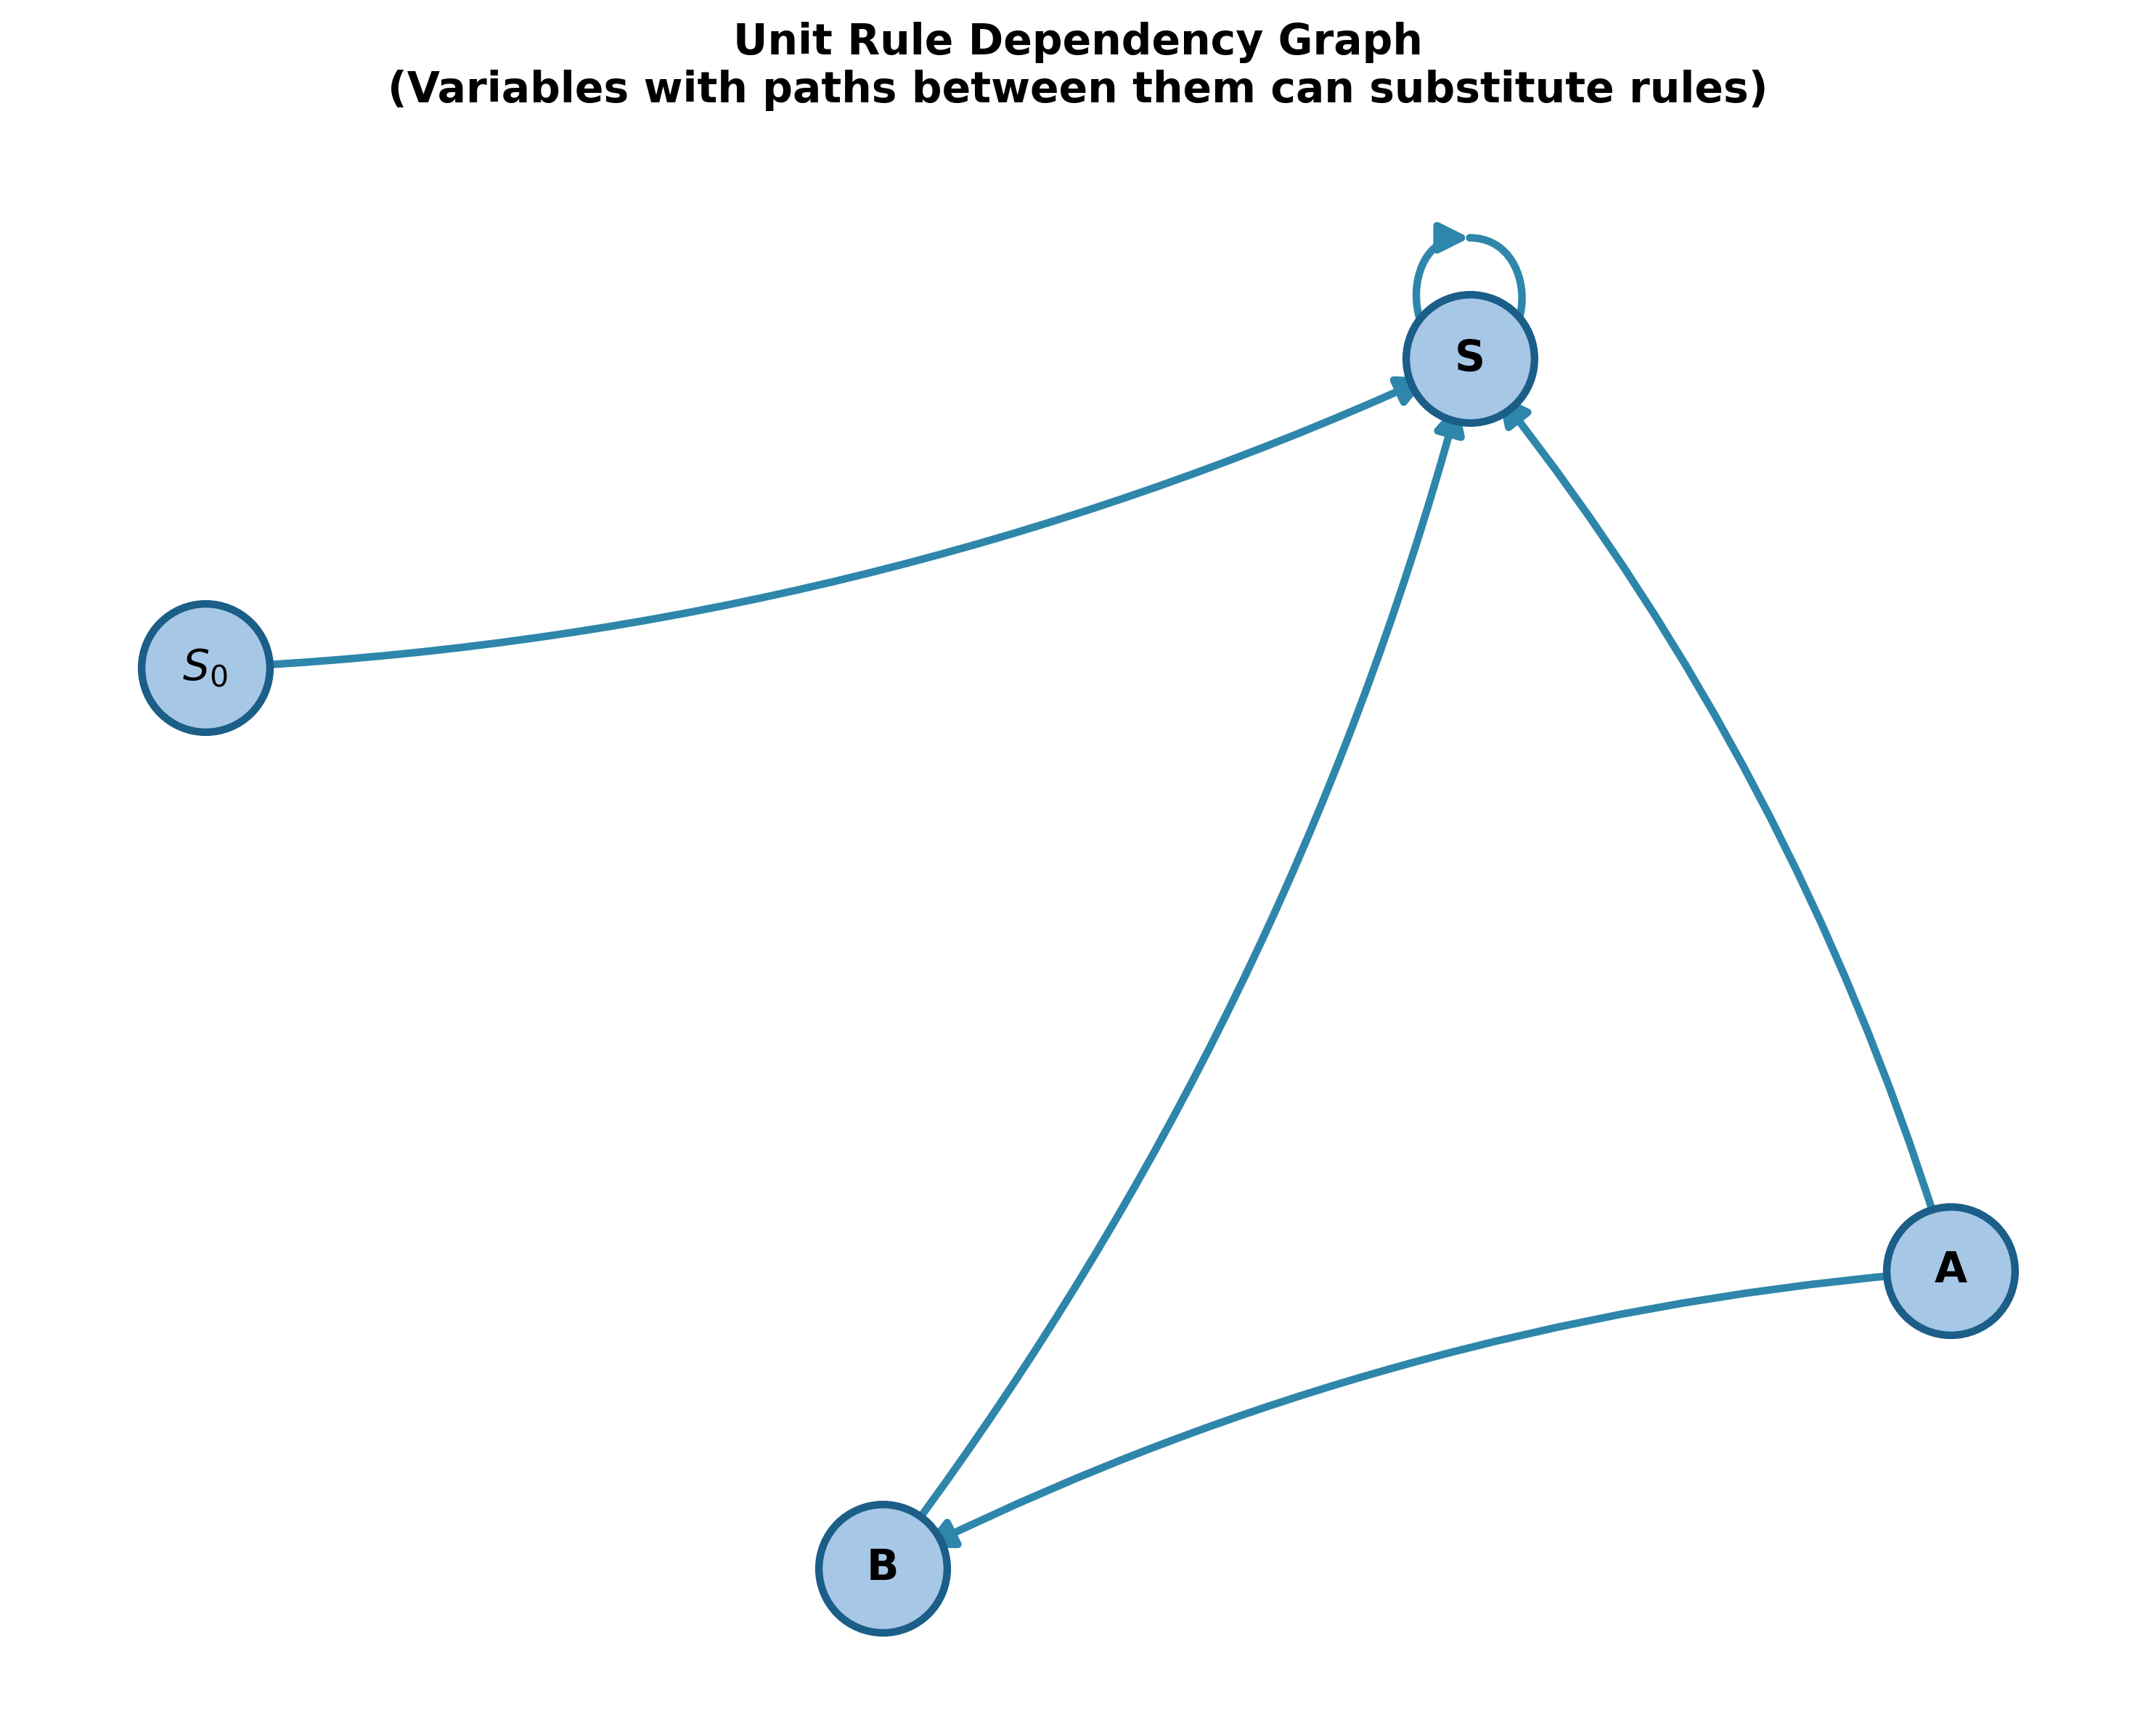
\includegraphics[width=0.7\linewidth]{phase2/chomsky_converter/out/directed_graph.png}
    \caption{\textbf{Unit Rule Dependency Graph.} Each arrow $A \to B$ means there's a unit rule from $A$ to $B$. If you can follow arrows from $X$ to $Y$, then $X$ can "borrow" all of $Y$'s non-unit productions.}
    \label{fig:dir_graph}
\end{figure}

\subsection{Step 3c: Follow All Paths (Using Floyd-Warshall)}

We use the \textbf{All-Pairs Shortest Path (APSP)} algorithm (specifically Floyd-Warshall) to find every pair of variables with a path between them.

\vspace{0.2cm}
\noindent\fbox{\parbox{\dimexpr\textwidth-2\fboxsep}{
\textbf{How it works:} For each pair $(X, Y)$:
\begin{itemize}
    \item If distance = $\infty$ $\rightarrow$ No path exists $\rightarrow$ Don't add anything
    \item If distance is finite $\rightarrow$ Path exists $\rightarrow$ Add all non-unit rules from $Y$ to $X$
\end{itemize}
}}

\vspace{0.3cm}

\noindent\textbf{Here's what we find by following the paths:}

{% for step in unit_elimination_steps %}
\begin{tcolorbox}[colback=blue!5!white,colframe=blue!75!black,title=Path Discovery \#{{ loop.index }}]
\textbf{From ${{step.from}}$ to ${{step.to}}$:}
\begin{itemize}
    \item \textbf{Path:} ${{step.from}} {% for node in step.path[1:] %} \to {{node}}{% endfor %}$
    \item \textbf{Distance:} {{step.distance}} step{% if step.distance != 1 %}s{% endif %}
    \item \textbf{Action:} Add these productions to ${{step.from}}$: \quad ${% for rule in step.rules_added %}{{rule}}{% if not loop.last %} \mid {% endif %}{% endfor %}$
\end{itemize}
\end{tcolorbox}
{% endfor %}

\subsection{Step 3d: Remove the Unit Rules Themselves}

After "copying over" all the necessary productions, we delete the unit rules themselves (shown in gray below). The dark yellow/orange rules were added from following unit rule paths:

\begin{align*}
    {% for variable, rules in unit_removed_grammar.items() -%}
    {%- set formatted_var = variable.replace('S0', 'S_0') -%}
    {{formatted_var}} &\to {% for rule in rules -%}
    {%- if rule in unit_rules_marked.get(variable, []) -%}
        \textcolor{gray}{${{- rule -}}$}
    {%- elif rule == 'e' -%}
        \varepsilon
    {%- else -%}
        {%- set is_new_rule = true -%}
        {%- if variable in e_removal_2_grammar and rule in e_removal_2_grammar[variable] -%}
            {%- set is_new_rule = false -%}
        {%- endif -%}
        {%- if is_new_rule -%}
            \textcolor{orange!80!black}{${{- rule -}}$}
        {%- else -%}
            {{- rule -}}
        {%- endif -%}
    {%- endif -%}
    {%- if not loop.last %} \mid {% endif -%}
    {%- endfor -%}
    \\
    {% endfor -%}
\end{align*}

\vspace{0.2cm}
\noindent\textcolor{green!60!black}{\textbf{\ding{51} Eliminate unit rules}}

{% else %}
\noindent\textbf{Good news!} This grammar doesn't have any unit rules, so we can skip this step entirely.

\vspace{0.2cm}
\noindent\textcolor{green!60!black}{\textbf{\ding{51} Eliminate unit rules (none present)}}
{% endif %}

\section{Step 4: Separate Terminals from Variables}

\subsection{Step 4a: The CNF Requirement}

In CNF, if a production has length greater than 1, it must contain \textit{only} variables—no terminals allowed. Productions like these violate this rule:
\begin{align*}
    A &\to aBC \quad \textcolor{red}{\textbf{\textsf{X}}} \text{ Mixes terminal $a$ with variables $B$ and $C$}
\end{align*}

\subsection{Step 4b: The Fix — Create Helper Variables}

\noindent\textbf{The Fix:} For each terminal that appears alongside variables, we create a new variable that "stands in" for that terminal:
\begin{align*}
    U_a &\to a \\
    U_b &\to b \\
    &\text{etc.}
\end{align*}

Then we can rewrite $A \to aBC$ as $A \to U_a BC$.

\subsection{Step 4c: After Applying This Transformation}

Rules with mixed terminals and variables are replaced with rules containing only variables. New helper variables $U_x$ are introduced for each terminal:

\begin{align*}
    {% for variable, rules in one_term_or_var_grammar.items() -%}
    {{variable.replace('S0', 'S_0')}} &\to {% for rule in rules -%}
    {% if rule == 'e' -%}
        \varepsilon
    {% else -%}
        {% if variable.startswith('U_') -%}
            \textcolor{green!50!black}{\textbf{ {{- rule -}} }}
        {% else -%}
            {{ rule }}
        {% endif -%}
    {% endif -%}
    {% if not loop.last %} \mid {% endif %}
    {%- endfor %}\\
    {% endfor -%}
\end{align*}

\vspace{0.2cm}
\noindent\textcolor{green!60!black}{\textbf{\ding{51} RHS is either one terminal or all variables}}

\section{Step 5: Break Up Long Productions}

\subsection{Step 5a: The Final CNF Requirement}

Productions with variables must have \textit{exactly two} variables on the RHS. No more, no less. Productions like these violate this rule:
\begin{align*}
    A &\to BCD \quad \textcolor{red}{\textbf{\textsf{X}}} \text{ Has three variables}
\end{align*}

\subsection{Step 5b: The Fix — Introduce Intermediate Variables}

\noindent\textbf{The Fix:} We break long productions into chains of two-variable productions:
\begin{align*}
    A &\to BCD \quad \text{becomes} \quad A \to BE \text{ and } E \to CD
\end{align*}

We process from left to right, pairing variables and creating intermediates as needed. If a pairing already exists in the grammar, we reuse it!

\subsection{Step 5c: Final Grammar in Chomsky Normal Form}

\begin{align*}
    {% for variable, rules in final_grammar.items() -%}
    {{variable.replace('S0', 'S_0')}} &\to {% for rule in rules -%}{{- "\\varepsilon" if rule == 'e' else rule -}}{% if not loop.last %} \mid {% endif %}{%- endfor -%}\\
    {% endfor -%}
\end{align*}

\vspace{0.2cm}
\noindent\textcolor{green!60!black}{\textbf{\ding{51} RHS has at most two variables}}

\section*{Verification: Is This Really CNF?}

Let's check our work! Every production in the grammar above has one of these forms:

\begin{center}
\begin{tabular}{|c|l|}
\hline
\textbf{Form} & \textbf{Description} \\
\hline
$A \to a$ & Single variable produces single terminal \\
$A \to BC$ & Single variable produces exactly two variables \\
\hline
\end{tabular}
\end{center}

\noindent\textbf{Success!} This grammar is in Chomsky Normal Form and is equivalent to the original grammar.

\vspace{0.3cm}
\noindent\fbox{\parbox{\dimexpr\textwidth-2\fboxsep}{
\textbf{What can we do with CNF?} Now that our grammar is in CNF, we can:
\begin{itemize}
    \item Use the \textbf{CYK (Cocke-Younger-Kasami) algorithm} to parse strings efficiently
    \item Easily determine if a string belongs to the language in $O(n^3)$ time
    \item Analyze the grammar's structure more systematically
\end{itemize}
}}